Fig.~\ref{fig:sketch} shows the sketch of the model, in which a large offshore solar panel floats on the sea surface in an infinite open area. Compared with the wave length, the structural length is so large that it can be seen as a infinite domain. The assumptions are that a). the structure is impenetrable for both the beneath water and the above air and b). vacuum does not occur. Therefore the solar panel can be modeled as a two-dimensional (2D) von K\'{a}rm\'{a}n plate that contains only the geometrical non-linearity. In the 2D case, the 1D Euler-Bernoulli-von K\'{a}rm\'{a}n beam models the geometrically non-linear structure. The linear potential theory describes the water motion and the hydrodynamics. A train of waves travelling in an arbitrary direction, e.g., rightwards, address the investigation of the fluid-structure interaction (FSI).

\begin{figure}
    % \centering
    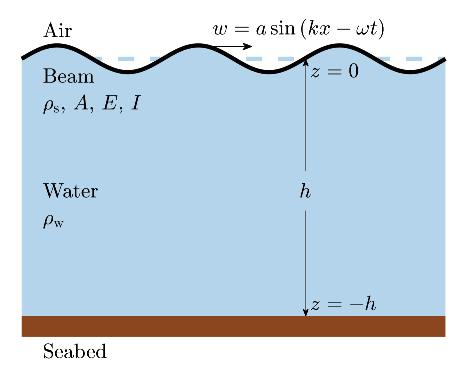
\includegraphics[width=0.5\columnwidth]{sketch.eps}
    \caption{A vary large ocean solar panel float on the sea surface. }
    \label{fig:sketch}
\end{figure}

\subsection{Governing equations}
\subsubsection{Nonlinear Euler-Bernoulli-von K\'{a}rm\'{a}n theory for beam}
The equation of motion (EOM) of the nonlinear Euler-Bernoulli-von K\'{a}rm\'{a}n beam reads
\begin{equation}
    \rho_\mathrm{s} A \pdv[2]{w}{t} 
    + E I \pdv[4]{w}{x} 
    - \frac{3}{2} A E \bkt{\pdv{w}{t}}^2\pdv[2]{w}{t}
    = q_\mathrm{w}.
    \label{eq: beam}
\end{equation}

The beam is of material density \ensuremath{\rho_\mathrm{s}}, cross-section area \ensuremath{A=bd}, Young's module \ensuremath{E} and inertial moment \ensuremath{I=\frac{bd^3}{12}}. Here \ensuremath{d} stands for the beam thickness (in \ensuremath{z}-direction), while \ensuremath{b} for the beam width (in \ensuremath{y}-direction that is neglected in 2D model). The water has density of \ensuremath{\rho_\mathrm{w}} and the uniform depth of \ensuremath{h}. \ensuremath{w} is the transverse displacement of beam. The external distributed load \ensuremath{q} is only the hydro-dynamic load because the floating equilibrium state sets off beam's gravity and buoyancy. \ensuremath{q} has the unit of \ensuremath{\Bkt{\si[per-mode=symbol]{\newton\per\meter}}} because the load is distributed over length in the 1D beam model.

\subsubsection{Liner potential theory for water}
The linear potential theory gives governing equations of inviscid, irrotational and incompressible fluid
\begin{equation}
    \pdv[2]{\phi}{x} + \pdv[2]{\phi}{z} = 0,
    \label{eq: laplace}
\end{equation}
where \ensuremath{\phi} represents the fluid velocity potential. 

At the bottom \ensuremath{z=-h}, the seabed is impenetrable: 
\begin{equation}
    \pdv{\phi}{z} = 0 \qq{at} z=-h,
    \label{eq: bottom}
\end{equation}
where \ensuremath{h} is the uniform water depth. 

At the free surface \ensuremath{z=0}, the kinematic boundary condition reads
\begin{equation}
    \pdv{\eta}{t} = \pdv{\phi}{z} \qq{at} z=0,
    \label{eq: surface kinematic bc}
\end{equation}
where \ensuremath{\eta} stands for the free surface elevation. And the Bernoulli equation gives the dynamic boundary condition:
\begin{equation}
    p + \rho_\mathrm{w} \pdv{\phi}{t} + \rho_\mathrm{w} \mathrm{g} \eta = 0 \qq{at} z = 0,
    \label{eq: surface dynamic bc}
\end{equation}
where \ensuremath{p} is the water pressure with unit \ensuremath{\Bkt{\si[per-mode=symbol]{\newton\per\meter\squared}}}, and \ensuremath{\mathrm{g}=\SI[per-mode=symbol]{9.81}{\Bkt{\meter\per\second\squared}}} is acceleration of gravity.

\subsubsection{FSI equations}
The beam and water models are coupled through the interface boundary conditions:
\begin{equation}
    w = \eta \qq{and} q_\mathrm{w} = p b \qq{at} z = 0.
    \label{eq: interface bc}
\end{equation}
Note that the force condition calculates the hydro-load by multiplying hydro-pressure \ensuremath{p} with beam width \ensuremath{b} for the consistence of unit \ensuremath{\Bkt{\si[per-mode=symbol]{\newton\per\meter}}}.

Now the fluid and structure governing equations are coupled at the free surface \ensuremath{z=0}:
\begin{equation}
    \pdv{w}{t} = \pdv{\phi}{z} 
    \label{eq: FSI kinematic}
\end{equation}
and
\begin{equation}
    \pdv[2]{w}{t} 
    + \beta \pdv[4]{w}{x} 
    - \frac{18\beta}{d^2} \bkt{\pdv{w}{t}}^2\pdv[2]{w}{t}
    + \alpha \pdv{\phi}{t} 
    + \alpha \mathrm{g} w 
    = 0,
    \label{eq: FSI EOM}
\end{equation}
where \ensuremath{\alpha} and \ensuremath{\beta} are two parameter ratios given by 
\begin{equation}
    \alpha = \frac{\rho_\mathrm{w}}{ \rho_\mathrm{b} d }
\end{equation}
and
\begin{equation}
    \beta = \frac{ d^2 E_\mathrm{b} }{ 12 \rho_\mathrm{b} }.
\end{equation}
Here, \ensuremath{A} \ensuremath{I} and \ensuremath{b} have been replaced or eliminated by \ensuremath{A=bd}, \ensuremath{I=\frac{bd^3}{12}} and Eq.~\eqref{eq: interface bc}.


\subsection{Non-dimensionalization}
Introduce new variables
\begin{equation}
    \left\{
    \begin{aligned}
        & X = k x \\
        & Z = k z \\
        & T = \sqrt{ k \tanh\bkt{kh} } \,  t \\
        & W\bkt{X,T} = \frac{w\bkt{X,T}}{a} \\
        & \Phi\bkt{X,Z,T} = \frac{ \sqrt{ k \tanh\bkt{kh} } }{ a \mathrm{g} } \phi\bkt{X,Z,T} \\
        & H = k h \\
        & \varepsilon = k a
    \end{aligned}
    \right.
    \label{eq: nondimensional variables}
\end{equation}
where \ensuremath{a} and \ensuremath{k} are the wave amplitude and wave number, respectively. The scaled time \ensuremath{T} is introduced partly for non-dimension (it is not completely dimensionless) and partly for easy multiplication. Note that the perturbation \ensuremath{\varepsilon} actually represents the wave steepness. 

Substitution of Eq.~\eqref{eq: nondimensional variables} into Eqs.~\eqref{eq: FSI kinematic} and \eqref{eq: FSI EOM} yields the non-dimensional EOM for the non-linear FSI governing equations at free surface \ensuremath{Z=0}:
\begin{equation}
    \pdv{W}{T} = \pdv{\Phi}{z}
    \label{eq: FSI kinematic nondimension}
\end{equation}
and
\begin{equation}
    k \tanh\bkt{H} \pdv[2]{W}{T}
    + \beta k^4 \pdv[4]{W}{X}
    - \varepsilon^2 18 \frac{ \beta k^2 }{ d^2 } \bkt{ \pdv{W}{X} }^2 \pdv[2]{W}{X} 
    + \alpha \mathrm{g} \pdv{\Phi}{T} 
    + \alpha \mathrm{g} W
    = 0
    \label{eq: FSI EOM nondimension}
\end{equation}

Eq.~\eqref{eq: FSI EOM nondimension} demonstrates that the non-linear term is of high order \ensuremath{\order{\varepsilon^2}}. In other words, the wave amplitude squared \ensuremath{a^2} scales the non-linearity. The non-linear effect become significant for the moderate-large waves, which suffices the requirement of the von K\'{a}rm\'{a}n theory. 

